% 
% Annual Cognitive Science Conference
% Sample LaTeX Paper -- Proceedings Format
% 

% Original : Ashwin Ram (ashwin@cc.gatech.edu)       04/01/1994
% Modified : Johanna Moore (jmoore@cs.pitt.edu)      03/17/1995
% Modified : David Noelle (noelle@ucsd.edu)          03/15/1996
% Modified : Pat Langley (langley@cs.stanford.edu)   01/26/1997
% Latex2e corrections by Ramin Charles Nakisa        01/28/1997 
% Modified : Tina Eliassi-Rad (eliassi@cs.wisc.edu)  01/31/1998
% Modified : Trisha Yannuzzi (trisha@ircs.upenn.edu) 12/28/1999 (in process)
% Modified : Mary Ellen Foster (M.E.Foster@ed.ac.uk) 12/11/2000
% Modified : Ken Forbus                              01/23/2004
% Modified : Eli M. Silk (esilk@pitt.edu)            05/24/2005
% Modified : Niels Taatgen (taatgen@cmu.edu)         10/24/2006
% Modified : David Noelle (dnoelle@ucmerced.edu)     11/19/2014

%% Change "letterpaper" in the following line to "a4paper" if you must.

\documentclass[10pt,letterpaper]{article}

\usepackage{cogsci}
\usepackage{comment}
\usepackage{pslatex}
\usepackage{apacite}
\usepackage{amsmath,amssymb}
\usepackage{graphicx}
\usepackage{subcaption}
\usepackage{color}
\usepackage{url}
\usepackage{todonotes}
\usepackage{mathtools}
\usepackage{stmaryrd}
\usepackage{booktabs}
\usepackage{array}
\usepackage{caption}
\usepackage{subcaption}
\usepackage{sidecap}
\usepackage[export]{adjustbox}
\hyphenpenalty=100000


\newcommand{\jefan}[1]{{\color{blue}{[jefan: #1]}}}
\newcommand{\kushin}[1]{{\color{orange}{[kushin: #1]}}}

\title{Semantic structure in communicative drawings}
 
% \author{\begin{tabular}[htbp]{c@{\extracolsep{1em}}c@{\extracolsep{1em}}c@{\extracolsep{1em}}c} \\
% {\large \bf Kushin Mukherjee} & {\large \bf Robert X. D. Hawkins} & {\large \bf Judith E. Fan}\\
% Department of Cognitive Science  & Department of Psychology & Department of Psychology \\ 
% Vassar College & Stanford University & Stanford University \\
% \texttt{kumukherjee@vassar.edu} & \texttt{rxdh@stanford.edu} & \texttt{jefan@stanford.edu} \\
% \end{tabular}
% }

% \author{{\large \bf Kushin Mukherjee\textsuperscript{1}, Robert X. D. Hawkins\textsuperscript{2}, Judith E. Fan\textsuperscript{2,3}} \\
% \textsuperscript{1}Department of Cognitive Science, Vassar College, \\
% \textsuperscript{2}Department of Psychology, Stanford University, \\
% \textsuperscript{3}Department of Psychology, University of California, San Diego}

\author{\large \bf Anonymous Authors}

\begin{document}

\maketitle 

\begin{abstract}

The ability to represent semantically meaningful structure in our environment is a powerful aspect of human visual perception and cognition. 
As a testament to this ability, we effortlessly grasp the correspondence between a drawing of a particular object and that physical object in the world, even if the drawing is far from realistic. 
How are visual object concepts organized such that they can robustly encode such abstract correspondences?
Here we explore the hypothesis that this is in part because we readily decompose both objects and drawings into a common set of semantically meaningful parts. 
Towards this end, we developed a web-based platform to densely annotate the semantic attributes of drawings of real-world objects produced in different contexts, allowing us to examine the semantic structure of more-detailed and sparser drawings of the same object. 
We found that: \textit{1}, people are highly consistent in how they interpret what individual strokes represent; \textit{2}, single strokes tend to correspond to single parts; \textit{3}, strokes representing the same part tend to be clustered in time; and \textit{4}, detailed and sparse drawings of the same object emphasized similar part information, although \textit{5}, detailed drawings of different objects tend to be more distinct from one another than simpler ones. 
Taken together, our results support the notion that people deploy their abstract understanding of the compositional part structure of objects in order to select actions to communicate relevant information about them in context. 
More broadly, they highlight the importance of structured knowledge for understanding how pictorial representations convey meaning. 

\textbf{Keywords:} 
sketch understanding; perceptual organization; visual production; object representation; compositionality
\end{abstract}

\section{Introduction}

%% revise so that the throughline is clearer: how does the human mind organize visual concepts such that they can be deployed so flexibly? answer: compositionality. what is a good way of probing compositionality? you could use discrimination tasks, but compositional tasks are much more direct. what is good about compositionality? it enables flexibility. how do you probe flexibility? compositional tasks across different contexts. 

When we open our eyes, we do not experience a meaningless array of photons --- instead, we parse the world into people, objects, and their relationships. 
The ability to represent semantically meaningful structure in our environment is a core aspect of human visual perception and cognition. 
As a testament to this ability, we effortlessly grasp the correspondence between a drawing of a particular object and that physical object in the world, even if the drawing is far from realistic. 
How are visual object concepts organized such that they can robustly encode such abstract correspondences?
Here we explore the hypothesis that this is in part because we readily decompose both objects and drawings into a common set of semantically meaningful parts. 

Recent advances in computational neuroscience and artificial intelligence have provided an unprecedentedly clear view into the algorithms used by the brain to extract semantic information from raw visual inputs, exemplified by modern deep learning approaches \cite{yamins2014performance}.
Nevertheless, a major gap remains in elucidating how the feature representations learned by deep learning models can be adapted to emulate the structure and flexibility of human visual semantic knowledge \cite{lake2017building}.
A promising approach to closing this gap may be to combine the learning capacity of deep neural networks with the parsimony and interpretability of structured representations that reflect how visual concepts are organized in the human mind \cite{battaglia2018relational}. 
Pursuing this strategy relies on a thorough understanding of this conceptual organization and how this organization enables behavioral flexibility.  

The goal of this paper is to contribute to this understanding by probing the expression of visual semantic knowledge in a naturalistic setting that exposes both its structure and flexibility: visual communication via drawing.
This approach departs from the conventional strategy for inferring the organization of visual object concepts from behavior, which relies upon tasks that elicit judgments about visual inputs, usually with respect to experimenter-defined dimensions. 
By contrast, visual communication tasks permit participants to include any elements they consider relevant to their goals and combine these elements freely, yielding high-dimensional information about how visual semantic knowledge is organized and deployed under a naturalistic task objective. 

Our aim in probing the semantic structure of communicative drawings is to shed light on how the semantic organization of visual object representations supports their flexible expression across contexts. 
Our approach advances recent work \cite{FanCommon2018,long2018drawings} that has investigated the production of object drawings to communicate in two ways: first, an explicit focus on compositional semantic structure in drawings, and second, the examination of flexibility in how visual semantic knowledge is expressed in different semantic contexts. 

Towards this end, we developed a web-based platform to densely annotate drawings of real-world objects produced in different semantic contexts, including detailed and simpler sketches of each object. 
Overall, we found that: (1) people are highly consistent in how they interpret what individual strokes represent; (2) single strokes tend to correspond to single parts; (3) strokes representing the same part tend to be clustered in time; and (4) detailed and sparse drawings of the same object emphasized similar part information, although (5) detailed drawings of different objects tend to be more distinct from one another than simpler ones. 
Taken together, our results support the notion that people deploy their abstract understanding of the compositional part structure of objects in order to select actions to communicate relevant information about them in context. 

\section{Methods}

\begin{figure}[htbp]
\centering
\includegraphics[width=0.48\textwidth]{figures/refgame_performance.pdf}
\caption{(A) Participants were paired in an online environment to play a drawing-based reference game in which the sketcher aimed to draw a target object such that a viewer could distinguish it from three distractor objects. (B) In close contexts, the target and distractors all belonged to the same basic-level category; in far contexts, the target and distractors belonged to different basic-level categories. (C) Sketchers used fewer strokes in the far condition, while producing sketches that were accurately recognized by the viewer in both conditions.}
\label{refgame_performance}
\end{figure}

% \noindent \textbf{Drawing dataset} \hspace{3mm} 

\subsection{Drawing dataset}
We obtained 1198 drawings of 32 real-world objects from a recent experimental dataset in which participants were paired in an online environment to play a drawing-based reference game \cite{fan2018modeling}.
Objects belonged to one of four basic-level categories (i.e., bird, car, chair, dog), each of which contained eight exemplars (Fig.~\ref{refgame_gallery}A).
On each trial of this reference-game experiment, both participants were presented with a shared context containing an array of photorealistic 3D renderings of four objects.   
One participant (i.e., the sketcher) aimed to draw one of these objects -- the target -- so that the other participant (i.e., the viewer) could pick it out from a set of distractor objects (Fig.~\ref{refgame_performance}A). 
Across trials, the similarity of the distractors to the target was manipulated, yielding two types of semantic context: close contexts, where the target and distractors all belonged to the same basic-level category, and far contexts, where the target and distractors belonged to different basic-level categories (Fig.~\ref{refgame_performance}B). 
This context manipulation led sketchers to produce simpler drawings containing fewer strokes and less ink on far trials than on close trials, while still achieving high recognition accuracy in both types of context (Fig.~\ref{refgame_performance}C, Fig.~\ref{refgame_gallery}B\&C). 
 
Prior work analyzing the semantic properties of such drawing data have represented them as rasterized images (e.g., \texttt{*.png}), an expedient format for applying modern convolutional neural network architectures \cite{FanCommon2018,sangkloy2016sketchy,yu2017sketch}. 
However, a key limitation of treating a drawing like an image is that one loses information about the inherently sequential and contour-based nature of drawing production. 
Because our goal is to characterize the fine-grained semantic organization of drawings, it was thus crucial for our purposes to represent each drawing instead using a vector image format (i.e., \texttt{*.svg}). 

Each drawing in our dataset is represented as a sequence of individual strokes, where each stroke consists of a sequence of sub-stroke elements, known as splines. 
These splines are parameterized as cubic Bezier curve segments, which are uniquely defined by four points: the initial point, the final point, and two control points that control the spline's curvature.
This data format provides a relatively compact representation of each drawing compared with a rasterized image, while still providing sufficient expressivity to provide an accurate representation. 

% The strokes that participants made on the canvas when creating the sketch can be represented as a concatenated string of cubic Bezier curves.  
% Thus, the final sketch can be represented by a list of such concatenated strings, each of which corresponds to an event of the participant placing their drawing instrument on the canvas, making some marks on the canvas, and lifting the instrument off of the canvas. 
% We were interested in collecting fine-grained annotations of these strokes, so we split strokes into sub-stroke elements, which we called splines. 
% A single spline was equivalent to a single cubic Bezier curve, i.e., a Bezier curve with two fixed end points and two control points to control curvature. 
% We had participants in our annotation task label each sketch's constituent splines.

\begin{SCfigure*}
\centering
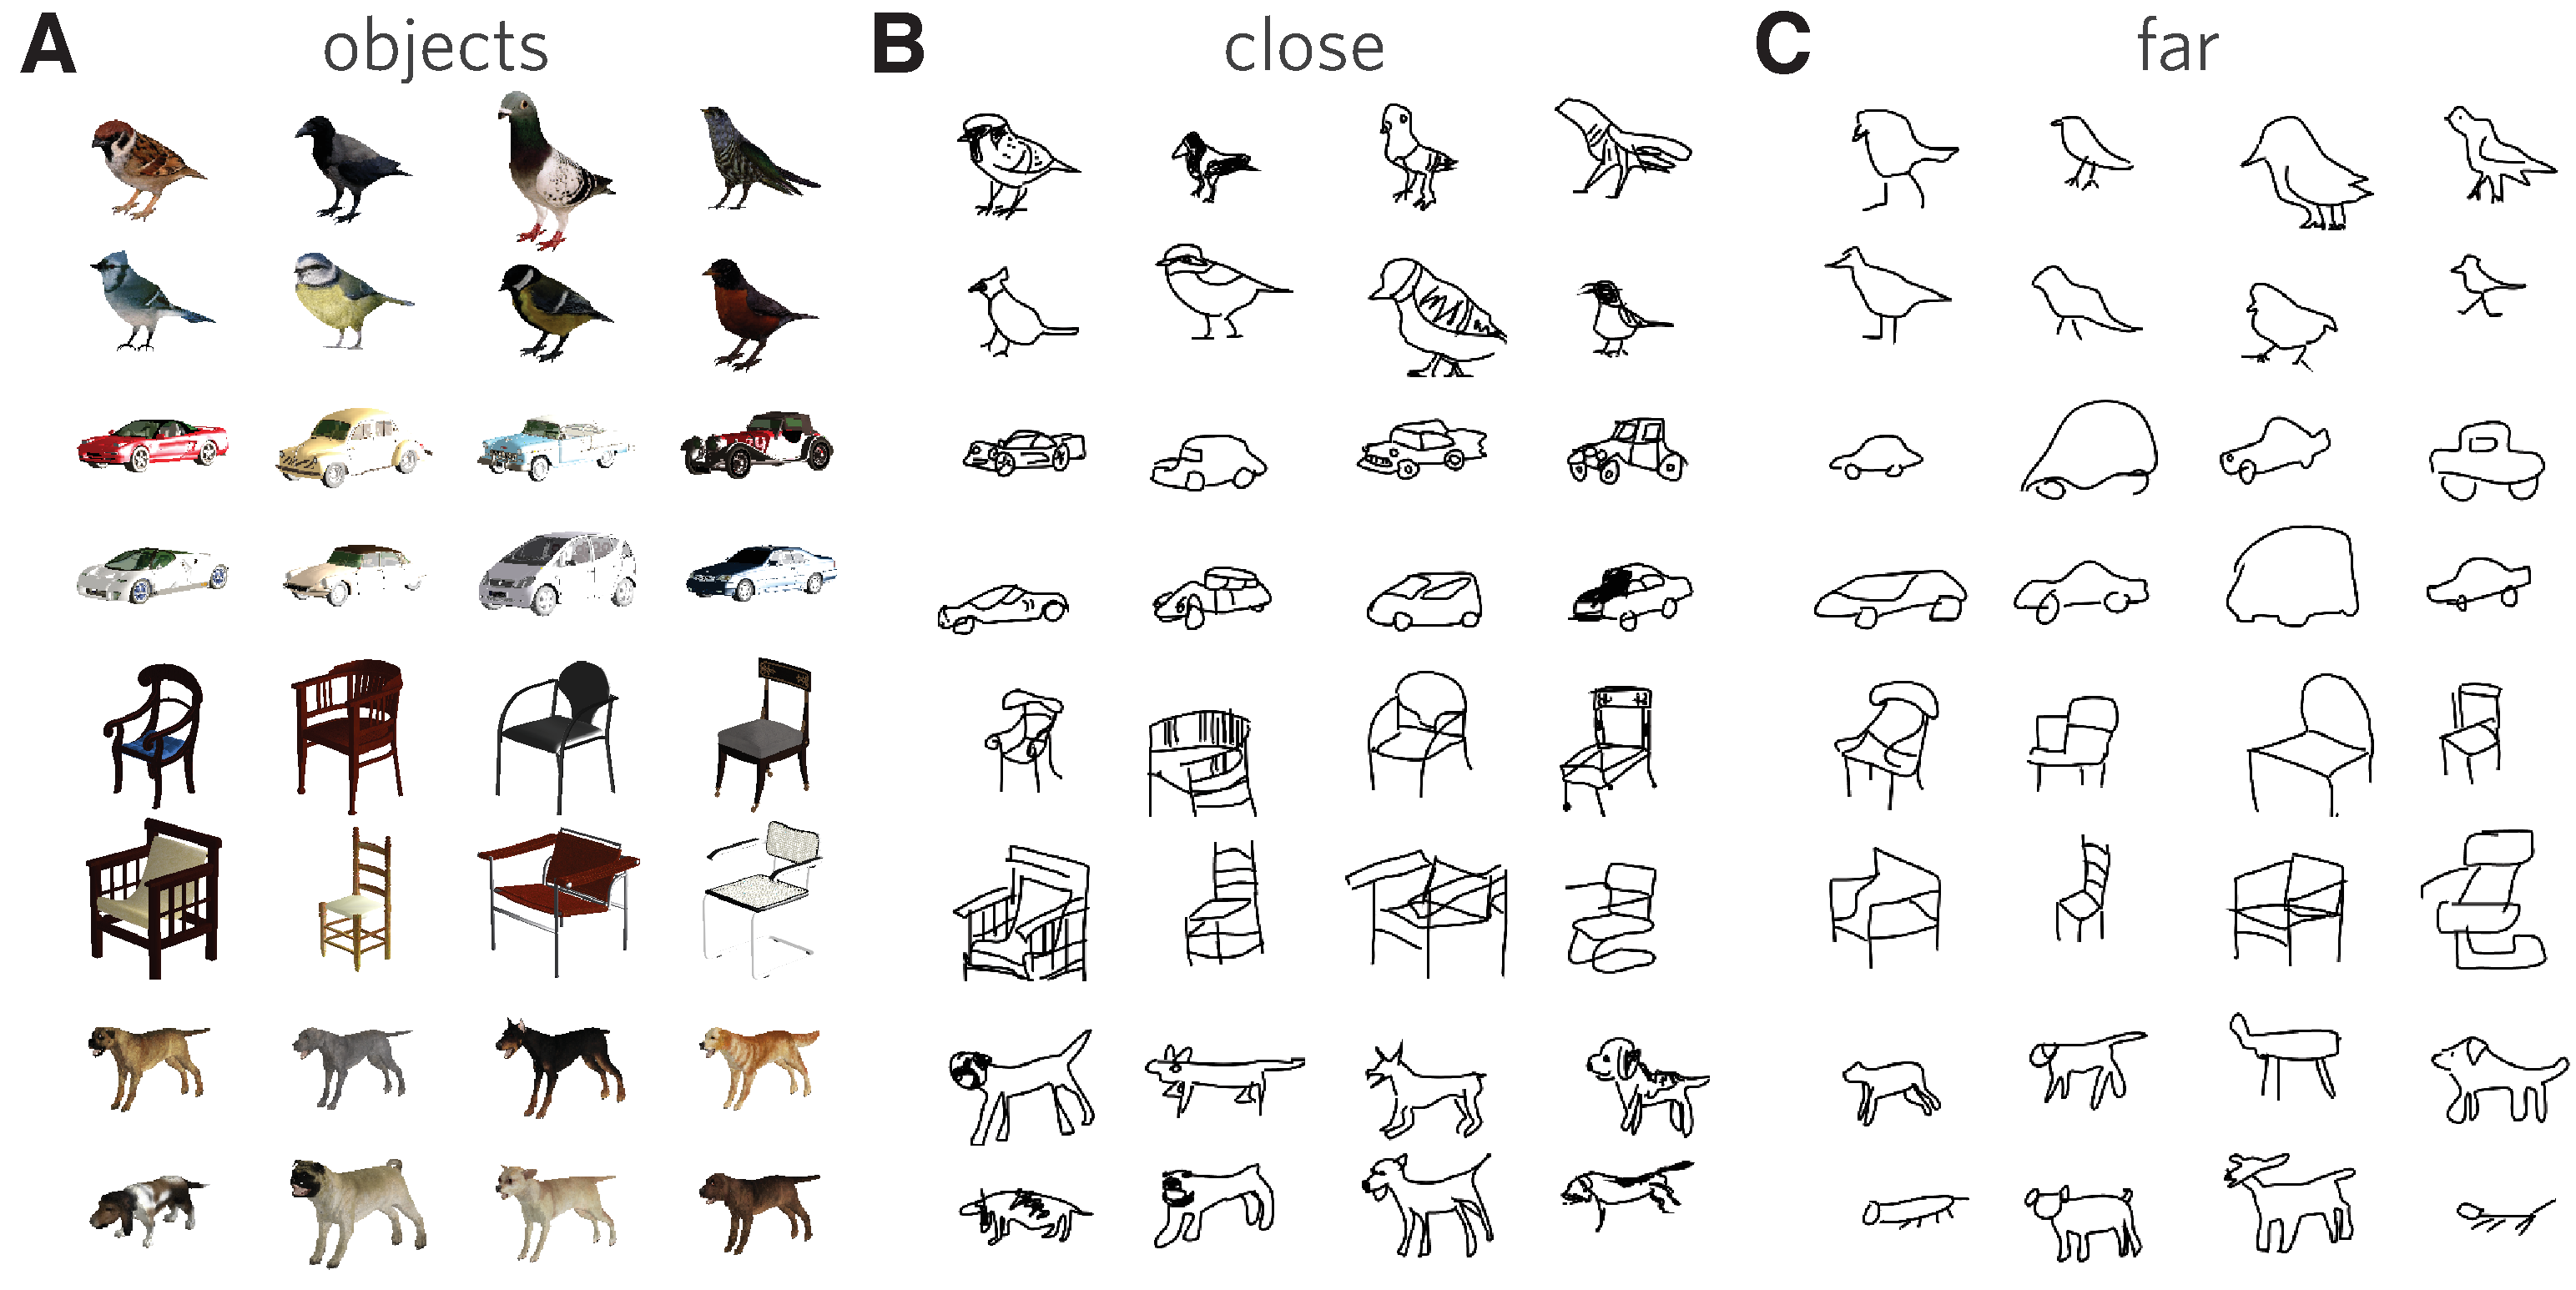
\includegraphics[width=0.8\textwidth]{figures/refgame_gallery.pdf}
\caption{(A) Target objects. (B) Example object drawings produced in a close context. (C) Example drawings produced in a far context.}
\label{refgame_gallery}
\end{SCfigure*}

\subsection{Semantic annotation}

In the present study, we developed a novel web-based platform to crowdsource semantic annotations for every spline of every stroke of every sketch in our dataset. 

\noindent \textbf{Participants} \hspace{3mm} 
326 participants were recruited via Amazon Mechanical Turk (AMT).  
For this experiment, participants provided informed consent in accordance with the Stanford University IRB. 
Participants were provided with a base compensation of \$0.35, plus \$0.002 for every sub-stroke element they annotated and \$0.02 for every sketch they annotated completely. 

\noindent \textbf{Annotation task} \hspace{3mm} \jefan{Would be good to put a cleaned up version of the annotation task interface around here.} In each annotation session, participants were presented with 10 drawings that were randomly sampled from the reference-game dataset. 
Each trial, one of these sketches appeared in the center of the display, above the same array of four objects that the sketcher had viewed, with one of these objects highlighted as the target. 
Thus the annotator had full information about which object the sketcher had intended to depict, as well as the identity of the distractors. 
The goal of the annotator was to tag each spline with a label corresponding to the part it represented (e.g., seat, leg, back for a chair). 
To facilitate this, participants were provided with a menu of common part labels that were tailored to each basic-level category represented in our dataset. \jefan{It would be good to have a table containing the part labels that were provided for each category.}
However, participants were also free to generate their own part label if none of the common labels applied.
In total, we collected 3608 annotation trials of 1195 unique sketches. \jefan{What happened to the other 3 drawings?}

% To collect fine-grained annotations of our drawings, we developed a web-based annotation tool. 
% Each participant annotated 10 sketches. 
% We provided participants with a sketch to be annotated on a canvas as well as a category-specific menu of labels, which they were encouraged to use for the annotation task. We also provided them with the option of entering their own labels through a free-response box. 
% The original set of images the sketcher had to discriminate between were shown to help the annotator better understand the contents of the sketch.
% Labeling was done by clicking on individual splines or clicking and dragging across multiple splines to highlight them before assigning them a label.
% Participants were encouraged to conduct their labeling of strokes in bouts — they were to highlight all the strokes corresponding to a single instance of a part before selecting a label from the menu. 
% Participants could do the task at their own pace and continue to a subsequent sketch whenever they felt they were ready. 
% They could choose to continue to the next trial without labeling every stroke in a sketch, but they would lose out on the completion bonus as well as the amount they would have earned for labeling the remaining strokes.
% In total, we collected 3608 annotations of 1195 unique sketches. 

\noindent \textbf{Inclusion criteria} \hspace{3mm} Because one of our central goals was to understand the relative emphasis that sketchers placed on different part information, we restricted our analyses to annotation trials in which the drawing was completely annotated (i.e., all splines were tagged). 
Moreover, in order to be able to examine inter-annotator consistency in how drawings were annotated, we only examined drawings that were annotated by at least three distinct participants. 
\jefan{By the way, are we including drawings that were annotated more than three times? We could, of course, and just ignore the 4th and onward... Also, have we ever checked whether the annotations were coming from distinct participants? Not sure, this requires comparing workerId, which we do not save to the group dataframe.}
Some of the custom part labels provided by participants were valid, but at a finer grain than the most frequently appearing labels. \jefan{Perhaps include an example of one of these.} 
In order to characterize the seamntic structure of drawings at a consistent granularity, we also manually constructed a part dictionary to map these overly fine-grained part labels to one of the common part labels, where appropriate. 
After applying these inclusion criteria, our annotated dataset consisted of 764 drawings that had been annotated exactly 3 times each, using a set of 24 unique part labels. 

% After collecting annotations, we filtered out any sketches that didn't have all of its constituent splines labeled. 
% This left us with 3319 annotations of 1190 unique sketches.
% Since there was some variability in the number of times each sketch in our dataset was annotated, we selected those sketches that had been annotated exactly 3 times. 
% This left us with 764 unique sketches, each of which had been annotated 3 times.
% We also created unique dictionaries for each object category that mapped participant-generated labels to the most frequently occurring labels in our dataset. 
% This helped reduce the total number of unique labels in our dataset from 228 to 24.

Given that our goal was to created an annotated dataset of sketches created under different contexts, we required that the annotations we collected through our interface be reliable. 
In order to assess this reliability, we looked at whether different annotators saw the same parts in these abstract sketches of objects. 
Specifically, we looked at inter-annotator reliability in spline labels between participants for each spline in our dataset. 
Reliability was measured in terms of 'agreement' on spline labels. 
For example, a 3/3 agreement score for a given spline meant that each of the 3 annotators applied the same label to that spline. 
We found that 67.85\% of splines in our dataset had 3/3 inter-annotator agreement, 27.77\% of splines had 2/3 agreement, and 4.38\% of splines had no agreement, which means that each participant applied a different label for each of those splines.
For the purposes of analysis, we set the modal label for each spline as its true label.

\section{Results}

\subsection{Relationship between strokes and parts}

\begin{figure}[htbp]
\centering
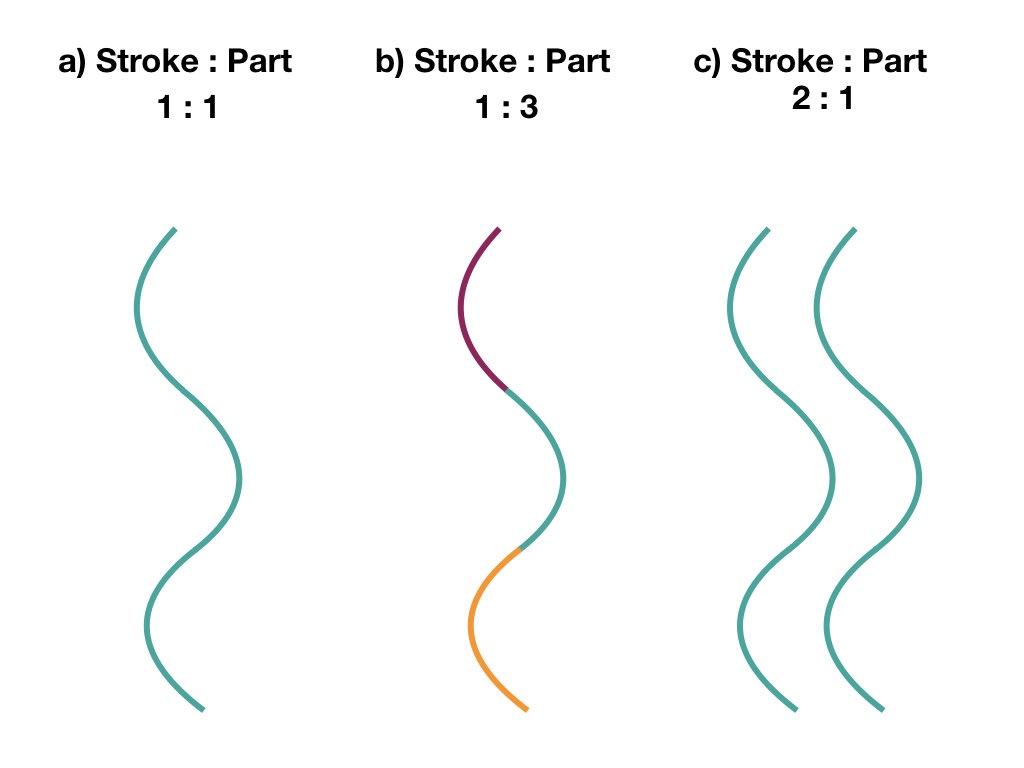
\includegraphics[width=0.5\textwidth]{figures/Part-Stroke.jpeg}
\caption{The three part-stroke relationships we explored. Each squiggle represents a hypothetical stroke. Different colors indicate different part-labels.}
\end{figure}

\begin{figure}[htbp]
\begin{subfigure}[t]{0.2\textwidth}
\centering
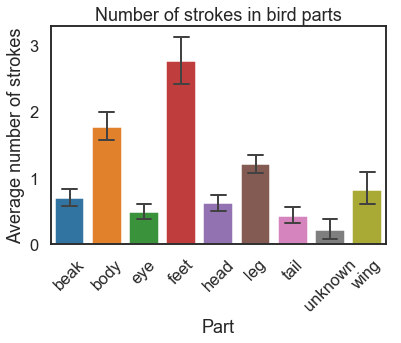
\includegraphics[width=1.2\textwidth]{figures/bird_average_parts.png}
\caption{Bird}
\end{subfigure}
 \hfill
\begin{subfigure}[t]{0.2\textwidth}
\centering
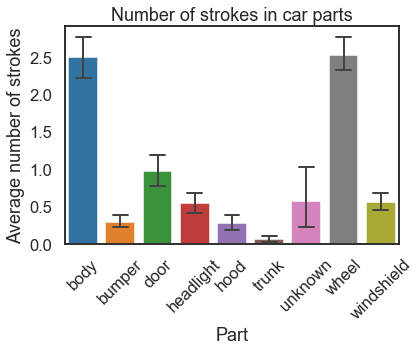
\includegraphics[width=1.2\textwidth]{figures/car_average_parts.png}
\caption{Car}
\end{subfigure}
\hfill
\begin{subfigure}[t]{0.2\textwidth}
\centering
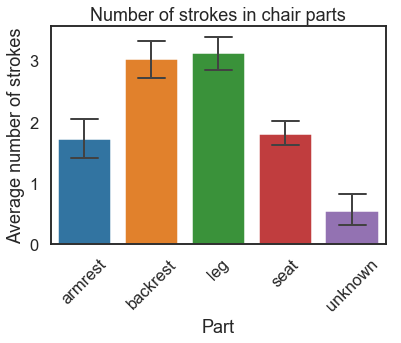
\includegraphics[width=1.2\textwidth]{figures/chair_average_parts.png}
\caption{Chair}
\end{subfigure}
 \hfill
\begin{subfigure}[t]{0.2\textwidth}
\centering
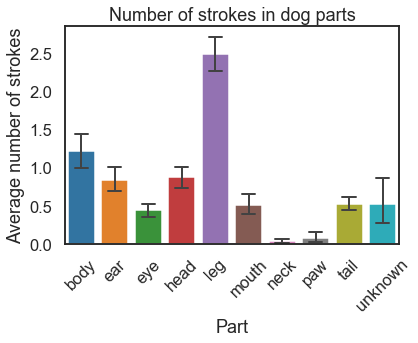
\includegraphics[width=1.2\textwidth]{figures/dog_average_parts.png}
\caption{Dog}
\end{subfigure}
\caption{Average number of strokes used to draw each part per category. While participants use multiple strokes to represent some parts, other parts are sometimes expressed using single strokes.}
\label{strokesperpart}
\end{figure}


People's hierarchical organization of visual concepts, such object category membership being determined by its constituent parts, allows for robust recognition of objects in the real world. 
We were interested in whether people might employ similar abstractions in producing sketches of such objects as well. 
Since an individual stroke correspond to a person's decision to make a mark on the canvas, we looked at the relationship between strokes and the parts that they represented in our dataset. 
We explored 3 possible stroke-to-part relationships:
a) Singular strokes correspond to singular parts, b) Singular strokes are used to convey multiple parts, that is, strokes cross semantic boundaries, and c) Multiple strokes are required to convey a single part. 

We compared a) and b) by looking at within-stroke label agreement for spline labels for all strokes in our dataset. High agreement among all the splines in a given stroke would be indicative of that being used to represent a single part. 
On the other hand, low agreement would indicate that stroke crosses semantic boundaries and is used to represent different parts. 
We found that splines contained in 76.85\% of strokes in our dataset shared a single label, 12.75\% of strokes contained 2 labels, and less than 11\% of strokes contained 3 or more labels. 
People, in general, tended to use their strokes to draw a single part while only sometimes utilizing a single stroke to represent multiple parts.

We also compared a) and c) by looking at the average number of strokes used to represent specific parts within a given category of sketches. 
A high average number of strokes for a given part would indicate that multiple strokes are utilized to draw that part, whereas a low average would indicate that a single or few strokes might suffice in depicting that part. 
Figure \ref{strokesperpart} shows these part-specific stroke averages by object category.
\kushin{I feel the above summary, including the figure caption for figure 2 is a little inconclusive. Thoughts on how to remedy this?}

\subsection{Stroke sequence organization}

\begin{figure}
\centering
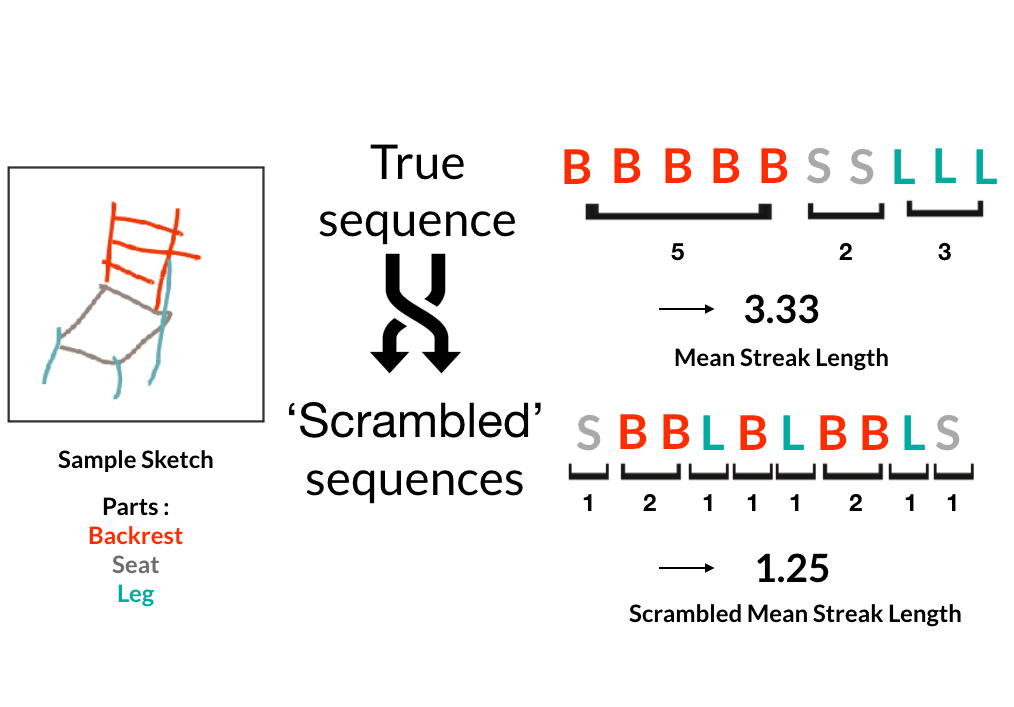
\includegraphics[width=0.5\textwidth]{figures/Part_sequence.png}
\caption{Analyzing stroke sequences in sketches. We first coded each stroke in our dataset in terms of its part label. Whenever multiple consecutive strokes that the sketcher had made shared a part-label, we counted the number of such strokes and termed it as a streak length for that part. This process was repeated for every stroke in a given sketch, after which we averaged over all the streak lengths for every part to obtain a single mean streak length value for every sketch in our dataset. To test whether strokes of the same part were reliably being drawn in bunches we scrambled the order of strokes in each sketch and calculating a 'scrambled' mean streak length. We repeated this scrambling process 1000 times to get a distribution of scrambled mean streak lengths for every sketch.}
\label{stroke_sequence_fig}
\end{figure}

Since individual strokes seemed to mostly correspond to singular part labels, we can view strokes as the building blocks for sketches much like words are the building blocks for sentences. Under this view of stroke organization, we looked at whether there was any meaningful temporal organization of strokes in terms of their part labels. If there was any such organization, any variation between the context conditions would also highlight a difference in how parts are mapped onto strokes under different communicative needs. This investigation was done through a permutation test approach where we created distributions of scrambled stroke sequences to test whether in the true sequence strokes of the same part were preferentially grouped together. Figure \ref{stroke_sequence_fig} outlines the procedure we undertook for this analysis.
74 sketches were excluded from this analysis because a) they consisted of only a single stroke, b) all the constituent strokes shared the same part label, or c) each stroke in the sketch had a unique label, making the permutation procedure not feasible.
We calculated the z-score of the true sequence of every sketch relative to their scrambled distributions. The higher this statistic was, the greater the amount of grouping of similar parts was relative to if the strokes were organized in a random fashion.

 The mean z-score for sketches in the close condition was 2.58 (95 CI: 2.26, 2.90) and 1.56 (95 CI: 1.38, 1.74) for the far condition.


 

% table for now: Is there spatial contiguity in how people structure their sketches?

\subsection{Modulation between communicative contexts}
\jefan{where we would report analysis of the sketch part features (num strokes, arc length)
e.g., when the far sketches are more abstract, how does that manifest in this feature representation?
like, are they more similar to each other, more like "bird" and lacking object-specific details?
a way of measuring this is that the centroid (euclidean norm, magnitude of the vector) is closer to the origin for far vs. close, and also that the RMSD to centroid of far sketches is smaller than for close sketches.... }



\section{Discussion}

\section{Acknowledgments}

\subsection{Tables}

\subsection{Figures}

\section{References}

\bibliography{semantic_parts}
\bibliographystyle{apacite}
\setlength{\bibleftmargin}{.125in}
\setlength{\bibindent}{-\bibleftmargin}ı




\end{document}
